\chapter{Moji podatki}
\label{ch:moji-podatki}

Grimove pravljice, volitve 2016 in slovenski geolocirani tviti so že pripravljeni podatki. Dodatek Text lahko nalaga podatke tudi iz drugih virov: Twitterja, Guardiana, New York Timesa in Wikipedie! 

Spodaj je primer, kako uporabiti gradnik Twitter.

\begin{figure}[h]
    \centering
    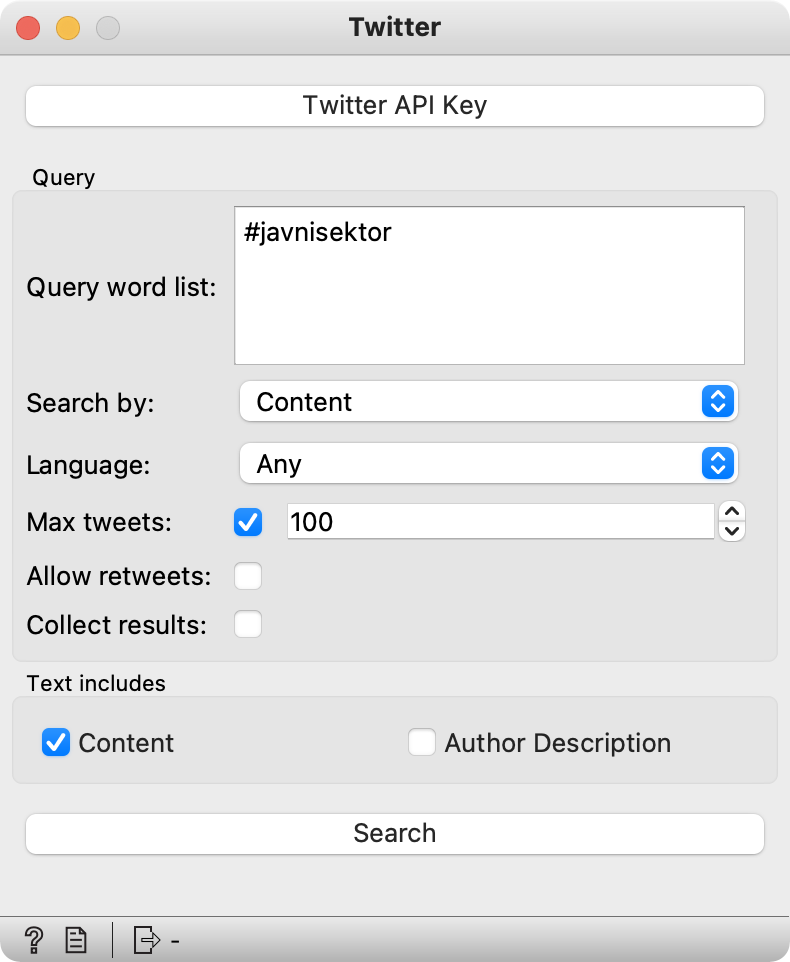
\includegraphics[width=0.65\linewidth]{twitter.png}%
    \caption{ }
    \label{fig:twitter}
\end{figure}

\begin{figure}[h]
    \centering
    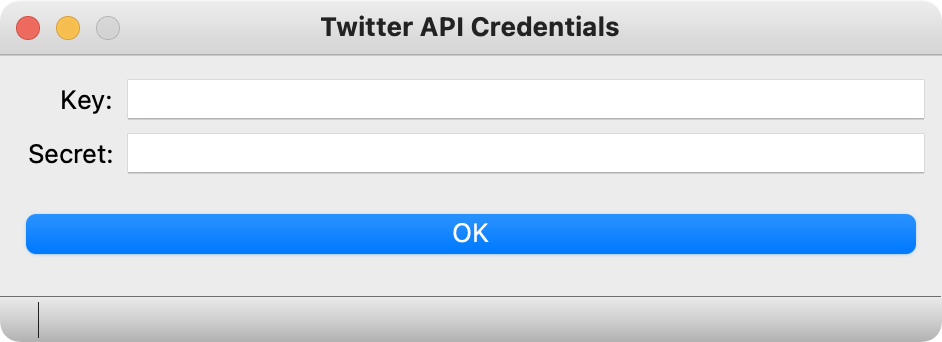
\includegraphics[width=0.65\linewidth]{key-window.png}%
    \caption{Za uporabo gradnika Twitter boste morali ustvariti svoj API ključ. Pojdite na \url{https://apps.twitter.com/} in ustvarite novo aplikacijo. S tem boste prejeli tudi svoj lasten API ključ. Vpišite podatke v okno Twitter API Key in pričnite z uporabo gradnika.}
    \label{fig:twitter-key}
\end{figure}

Odprite gradnik \textit{Twitter}. Prenesli bomo sto angleških tvitov z oznako \#javnisektor. Iskalni ukaz smo vnesli v polje \textit{Query word list} in nastavili jezik na angleščino.

\begin{marginfigure}[0cm]
    
\includegraphics[width=\linewidth]{twitter-workflow.png}
    \caption{}
\end{marginfigure}

Ko pritisnemo gumb \textit{Search} bo gradnik poiskal podatke in jih dal na izhod. Povežite Twitter z gradnikom Corpus Viewer in poglejte, kaj smo prenesli.

Twitter (in drugi podobni gradniku) omogočajo, da sami ustvarite nabor podatkov in jih uporabite za analizo. Preizkusite katerega izmed delotokov na novih podatkih!